% !TEX root = ../my-thesis.tex
%
\chapter{Approach}
\label{sec:approach}

In this chapter the two alternatives considered in this thesis to tackle the problem of ranking classification algorithms regarding properties of the data set. First, the theoretical approach is presented. Then, implementation details are discussed.

\section{Theory}

In general, the aim is to predict a ranking of algorithms based on properties, or meta features of a data set. This means, that as training data for a ranking approach (ranker), a number of performance values of classifiers need to be recorded on data sets in a first pre-processing phase, for which also meta features are to be computed. The table of this collected data is illustrated in Table \ref{tab:performanceValues}, for n meta features, k classifiers and n data sets. This approach to ranking is realized here, as pointed out before, in a regression based and preference based approach, which are explained in detail in the following sections.

\begin{table}[h]
\centering
	\begin{tabularx}{\textwidth}{X | X | X | X | X | X | X | X}
		%\hline
		MF 1			& MF 2		& ... 	& MF n		& PV 1 		& PV 2 		&	...	&	PV k 		\\ \hline
		$v_{11}$		& $v_{12}$	& ...	& $v_{1n}$	& $p_{11}$	& $p_{12}$	& 	...	&	$p_{1k}$		\\ 
		$v_{21}$		& $v_{22}$	& ...	& $v_{2n}$	& $p_{21}$	& $p_{22}$	& 	...	&	$p_{2k}$		\\ 
		...			& ...		& ...	& ...		& ...		& ...		&	...	&	...			\\ 
		$v_{m1}$		& $v_{m2}$	& ... 	& $v_{mn}$	& $p_{2m}$	& $p_{m2}$	& 	...	&	$p_{mk}$			 
	\end{tabularx}
	\label{tab:performanceValues}
	\caption{Training data for the rankers.}
\end{table}

\subsection{Regression Based Ranking}
% How is the regression ranking done
One possibility to derive a ranking of classifiers from this information when given a new data set is to use regression models. The idea is to use separate regression models to predict a performance value for each classifier, and to then derive an ordering from these predictions. This is done by splitting the data set compiled beforehand (see Tab. \ref{tab:performanceValues}) into separate data sets that each contain all meta features for all data sets, but only the performance values of one classifier, as illustrated in Table \ref{tab:regressionTables}. The target feature on these individual data sets, the performance value of the classifier, is a numeric value, and thus a regression model can be trained on each of them. All regression models therefore try to learn the target function metafeatures$\rightarrow$performance value for their respective classifier. Hence for a query instance, after computing the meta features, these are fed into each regression model and the predicted performance value for each classifier is saved. In a second step, the classifiers are ordered according to the predictions. This process the ranker passes through for making a prediction is presented in Figure \ref{fig:regression_ranker_model}.

\begin{table}[h]
\centering
\resizebox{\textwidth}{!}{%
	\begin{tabularx}{1.1\textwidth}{X | X | X | X}
		%\hline
		Meta Feature 1	& ... 	& Meta Feature n		& Performance Value 1	\\ \hline
		$v_{11}$			& ...	& $v_{1n}$			& $p_{11}$				\\ 
		$v_{21}$			& ...	& $v_{2n}$			& $p_{21}$				\\ 
		...				& ...	& ...				& ...					\\ 
		$v_{m1}$			& ... 	& $v_{mn}$			& $p_{m1}$				\\ \hline\hline
		Meta Feature 1	& ... 	& Meta Feature n		& Performance Value 2 	\\ \hline
		$v_{11}$			& ...	& $v_{1n}$			& $p_{12}$				\\ 
		$v_{21}$			& ...	& $v_{2n}$			& $p_{22}$				\\ 
		...				& ...	& ...				& ...					\\ 
		$v_{m1}$			& ... 	& $v_{mn}$			& $p_{m2}$					 
	\end{tabularx}
}	
\vspace{1em}
...
\vspace{1em}	
\resizebox{\textwidth}{!}{%
	\begin{tabularx}{1.1\textwidth}{X | X | X | X}
		%\hline
		Meta Feature 1	& ... 	& Meta Feature n		& Performance Value k 	\\ \hline
		$v_{11}$			& ...	& $v_{1n}$			& $p_{1k}$				\\ 
		$v_{21}$			& ...	& $v_{2n}$			& $p_{2k}$				\\ 
		...				& ...	& ...				& ...					\\ 
		$v_{m1}$			& ... 	& $v_{mn}$			& $p_{mk}$					 
	\end{tabularx}
}
	\caption{How the regression ranker processes the training data.}
	\label{tab:regressionTables}
\end{table}

\begin{figure}
\centering
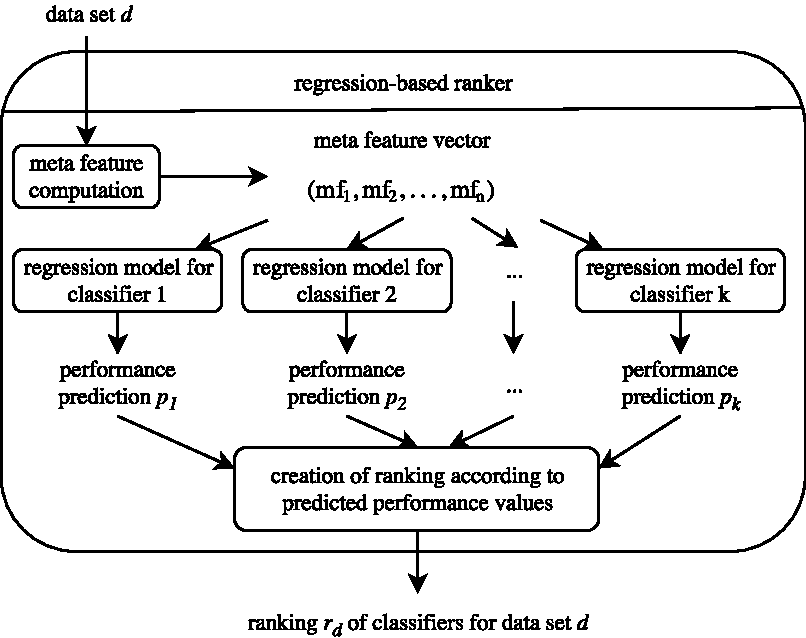
\includegraphics[scale=1]{gfx/regression_models.pdf}
\caption{An overview of how a regression based ranker constructs a ranking.}
\label{fig:regression_ranker_model}
\end{figure}

\subsection{Preference Based Ranking}
% How is the preference ranking done
The second possibility considered in this context is using preference learning to predict a ranking. Each instance of the data set generated beforehand (see Fig \ref{tab:performanceValues}) contains meta feature information for the considered data set and performance values of all classifiers. Similar to the regression alternative, the performance values can be converted to preference information by sorting the corresponding classifiers by their performance values for each data set. This leads to an ordering of classifiers associated with each instance, and implies that the preference learning task at hand is label ranking. In this case, there exists only one label ranking model which is fed the computed meta data for a new data set and returns an ordering of classifiers, which is depicted in Figure \ref{fig:preference_ranker_model}. Thereby it attempts to learn the mapping from meta features to an ordering of classifiers directly.

\begin{table}[h]
\centering
	\begin{tabularx}{\textwidth}{X | X | X | X | X}
		%\hline
		MF 1				& MF 2				& ... 	& MF n				& Ranking 	\\ \hline
		$v_{11}$			& $v_{12}$			& ...	& $v_{1n}$			& $r_1$		\\ 
		$v_{21}$			& $v_{22}$			& ...	& $v_{2n}$			& $r_2$		\\
		...				& ...				& ...	& ...				& ...		\\
		$v_{m1}$			& $v_{m2}$			& ... 	& $v_{mn}$			& $p_m$		 
	\end{tabularx}
	\label{tab:preferenceTable}
	\caption{How the preference ranker processes the training data.}
\end{table}

\begin{figure}
\centering
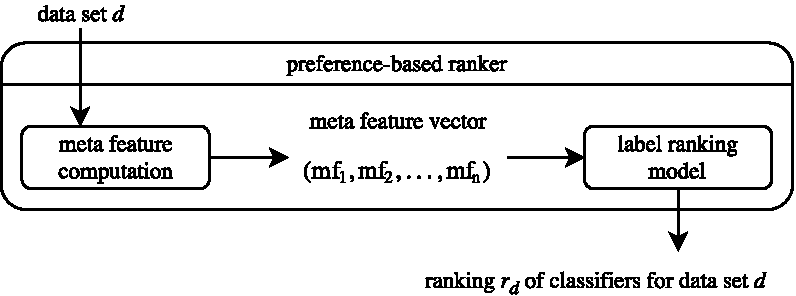
\includegraphics[scale=1]{gfx/label_ranking_model.pdf}
\caption{An overview of how a preference based ranker constructs a ranking.}
\label{fig:preference_ranker_model}
\end{figure}

\section{Implementation}
In general, all implementations for the approach are carried out in Java, particularly Java 8. However, some additional packages where used, which are pointed out briefly. For the implementation of the regression models, WEKA was used, a popular libary of machine learning algorithms that includes algorithms for classification, regression, and provides help in the evaluation of these learning algorithms \cite{hall2009weka}. Regarding the preference algorithms, the jPL framework was used \cite{intelligent2017jpl}. The jPL framework is a java framework for the evaluation of preference learning algorithms, it implements several tasks from the context of preference learning, including label ranking, and also provides a representation for data sets that contain label ranking information. The list of meta features used is taken from OpenML \cite{OpenML2013}, a website that not only provides a large number of openly accessible data sets, but also records performance values of learning algorithms on these data sets, and features properties of data sets. Thus the meta features where calculated with the help of an implementation provided by OpenML in its Evaluation Engine \cite{openMLEvaluationEngine}; The full list of meta features is included in Table \ref{tab:metaFeatureDetails} in the Appendix.